% Formato modificado por CORUM para la escritura de artículo

% Si es formato ieee descomentar la siguiente linea
%\documentclass[conference]{IEEEtran_ES}

% Si es formato a una columna descomentar la siguiente linea
%\documentclass[11pt,a4paper,onecolumn]{article}
\documentclass[a4paper]{article}

\usepackage[utf8]{inputenc}
%\usepackage[latin1]{inputenc}
\usepackage[spanish]{babel}
\usepackage{amsmath}
\usepackage{amsfonts}
\usepackage{amssymb}
\usepackage{graphicx}
\usepackage{natbib}
\usepackage[colorlinks,hyperindex,linkcolor=red,urlcolor=blue]{hyperref}
\usepackage{setspace}

\usepackage{epsfig}
%\usepackage{array}
%\usepackage{times}
%\usepackage{multibib}

%ruta para guardar las imagenes
\graphicspath{ {figuras/} }

%manejo de margenes (comentar si no es IEEE)
\setlength{\topmargin}{-30.0 pt}
\setlength{\headsep}{50.0 pt}
\setlength{\textwidth}{6,25 in}
\setlength{\textheight}{9.0 in}
\setlength{\oddsidemargin}{0 in}
\setlength{\evensidemargin}{0 in}
\setlength{\marginparwidth}{0 in}
\setlength{\marginparsep}{0 in}


\begin{document}
\title{Plataforma educativa de sexualidad ``Red Sentir... Con-ciencia juvenil''}

% sin IEEE
\author{J. A. Gómez Múnera$^{\ast }$ y A. Giraldo$^{\ast }$}
\date{$^{\ast }$Corporación Estudiantes Universitarios y Profesionales de Marinilla (CORUM)
\\Calle 30 San José N$\circ$ 25-118, Marinilla - Antioquia, Colombia
\\ \href{mailto:gomezmunera@corum.org.co}{gomezmunera@corum.org.co}, \href{mailto:alejo@corum.org.co}{alejo@corum.org.co}}


% make the title area
\maketitle

%\renewcommand{\abstractname}{Abstract}
\renewcommand{\tablename}{Tabla}
\renewcommand{\refname}{REFERENCIAS}

\abstract Dentro del plan nacional de desarrollo 2014-2018 de Colombia se planteó la educación como un pilar fundamental, que sirviera como un mecanismo que permitiera una igualdad social al permitir nivelar las posibilidades de todos los Colombianos. Teniendo esto en cuenta, y al considerar el incremento acelerado en el uso de las tecnologías de la información y la comunicación, junto con la posibilidad de brindar una mayor cobertura en educación, que la corporación de estudiantes universitarios y profesionales de Marinilla (CORUM) desarrolló e implementó un proyecto llamado ``Red Sentir...Con-ciencia juvenil'' centrado en la prevención de embarazo adolescente, fortalecimiento del plan de vida, pensamiento crítico, autonomía y toma de decisiones consientes. El proyecto se deriva en tres componentes fundamentales que constituyen un proceso de formación integral con jóvenes entre 10 y 19 años del oriente Antioqueño, que les permite interactuar y relacionarse con padres, maestros y agentes institucionales. Los componentes relacionados son: (i) formación y socialización, (ii) mesa regional, y (iii) una plataforma digital. El presente artículo hace énfasis en las estrategias y desarrollos del componente digital para vincular la educación sexual, los derechos sexuales y reproductivos, el acceso a métodos anticonceptivos y la interacción con expertos. Para el desarrollo se creó una red social a través de diferentes tecnologías, que involucran desarrollo web, creación de bases de datos relacionales, configuración de servidores y desarrollo de videojuegos. Todas esto posible a través de distintos lenguajes de programación tales como, python, HTML, javascript, que configuran aplicaciones tanto desde el lado del cliente como aplicaciones desde el lado del servidor.\endabstract

\noindent{\textbf{Keywords:}} Plataforma educativa, embarazo adolescente, Oriente Antioqueño, desarrollo web, desarrollo de videojuegos.\newline

\section{INTRODUCCIÓN}

Uno de los temas prioritarios que enfrentan los países es lograr una inclusión social, en particular en los jóvenes que se encuentran en situación de pobreza y vulnerabilidad, ya que ellos son quienes pueden llegar a tomar comportamientos de riesgo que puedan provocar en la mayoría de casos conflictos relacionados la deserción escolar o embarazos a temprana edad, lo que suscita que los ciclos de pobreza se perpetúen.

En~\citep{BID2017} se menciona un marco sectorial de protección social y pobreza (GN-2784) del BID, en el que se marcan la importancia de la prestación de servicios de inclusión social (enfoque objetivo) para adolescentes que puedan estar en riesgo, buscando fomentar en ellos la autonomía (enfoque subjetivo) que les permita desempeñar papeles relevantes dentro de su propio contexto. El garantizar que los jóvenes puedan tener y acceder a estos servicios es importante para evitar los factores de riesgo que pueden interrumpir la construcción del individuo hacia una vida adulta y productiva. Por ende, cuando se analizan las características que intervienen en la inclusión social, lleva consigo a tener en cuenta la exclusión social, ocasionado por factores estructurales, así también de acuerdo a las características individuales de los jóvenes. Al enlazar esto con las políticas de los países para reducir la problemática de embarazo adolescente, si no se asegura la disponibilidad y acceso
efectivo de los y las adolescentes a métodos anticonceptivos (factores estructurales), cualquier otra acción que se realice tendrá efectos limitados. De la misma manera, aunque estén a disposición y sean accesibles los métodos anticonceptivos, la probabilidad de uso efectivo, consciente y consistente aumenta si su distribución viene acompañada de un proceso de formación sobre salud sexual y salud reproductiva. Todo lo anterior lleva a pensar, que para llevar a cabo estrategias de intervención verdaderamente efectivas deben tenerse en cuenta tanto los factores estructurales como los factores de riesgo que actúan en los adolescentes, en la medida que puedan ser llevadas a cabo simultáneamente consolidan todo el proceso de intervención para alcanzar resultados significativos que perduren en el tiempo, en caso contrario, cuando los esfuerzos se realizan de manera independiente se disminuye la efectividad de la estrategia y posibilidad de que sea autosostenible.

Estas estrategias pueden ser abordadas desde un enfoque de derechos, los cuales constituyen las condiciones estructurales mencionadas para permitir a los adolescentes un contexto de garantías para un desarrollo pleno, el no contar con estas garantías o al presentarse en una situación de exclusión puede llevar al adolescente en términos de sexualidad a tener relaciones sexuales con falta de información veraz y clara, sin protección, ocasionado embarazos a temprana edad o riesgos de contraer infecciones de transmisión sexual. 

En Colombia la  fecundidad  en  la  adolescencia  se  convirtió  en  un problema de salud pública cuando a partir de 1990 para adolescentes entre 15 y 19 años es de $12.8\%$, y se  detecta  su  tendencia  sistemáticamente  creciente  que encuentra  el  valor  máximo  en  2005 ($20.5\%$). Para el año 2010 ($19.5\%$) se logró una tendencia decreciente que se continua presentando en el 2015 con una medida del $17.4\%$ (En la figura~\ref{fig:ends} se muestra las mediciones y las diferencias por desagregaciones geográficas o socioeconómicas), y que se espera que para el año 2021 según el ajuste realizado al Plan Decenal de Salud Pública 2012-2021 disminuir ese porcentaje a un $15\%$~\citep{Pro2015}.

Colombia se planteo en los objetivos de desarrollo del milenio (ODM) tener tazas de embarazo adolescente por debajo del $15\%$, sin embargo los porcentajes alcanzados fueron muy alejados de esas cifras, por lo cual es necesario redoblar los esfuerzos que permitan disminuir embarazo en adolescentes. En 2013 Colombia registró 6.423 nacimientos de mujeres entre los 10 y 14 años y casi 150 mil de mujeres entre los 15 y 19 años, cifra que es elevada si se tiene en cuenta que en conjunto representan el $23.5\%$ del total de nacimientos~\citep{PNUD2015}.

Los esfuerzos por reducir el embarazo adolescente han sido más significativos en los grupos más favorecidos socialmente, esto en contraposición de los menos favorecidos que han tenido un descenso menos significativo que ha provocado que se amplíen las brechas socioeconómicas. Esto refleja la  necesidad de realizar mayores esfuerzos de la política de prevención del embarazo adolescente en los grupos menos favorecidos socialmente: zonas rurales, menos educados, situaciones de pobreza. 

Las diferencias ocasionadas por las situaciones socioeconómicas y por la ubicación geográfica, ponen en evidencia que se deben tomar acciones o generar estrategias de inclusión social, en el que se aborden las temáticas de educación sexual de manera transversal con un enfoque de derechos y con una mayor cobertura, para permitir así la reducción de las brechas existentes confirmadas en el plan nacional de desarrollo 2014-2018, y  el  principio  de  “no  dejar  a  nadie  atrás”  consagrado  en  la  Agenda  2030,  que  comprende a los Objetivos de Desarrollo Sostenible (ODS).
	
\begin{figure}[t]
\centering
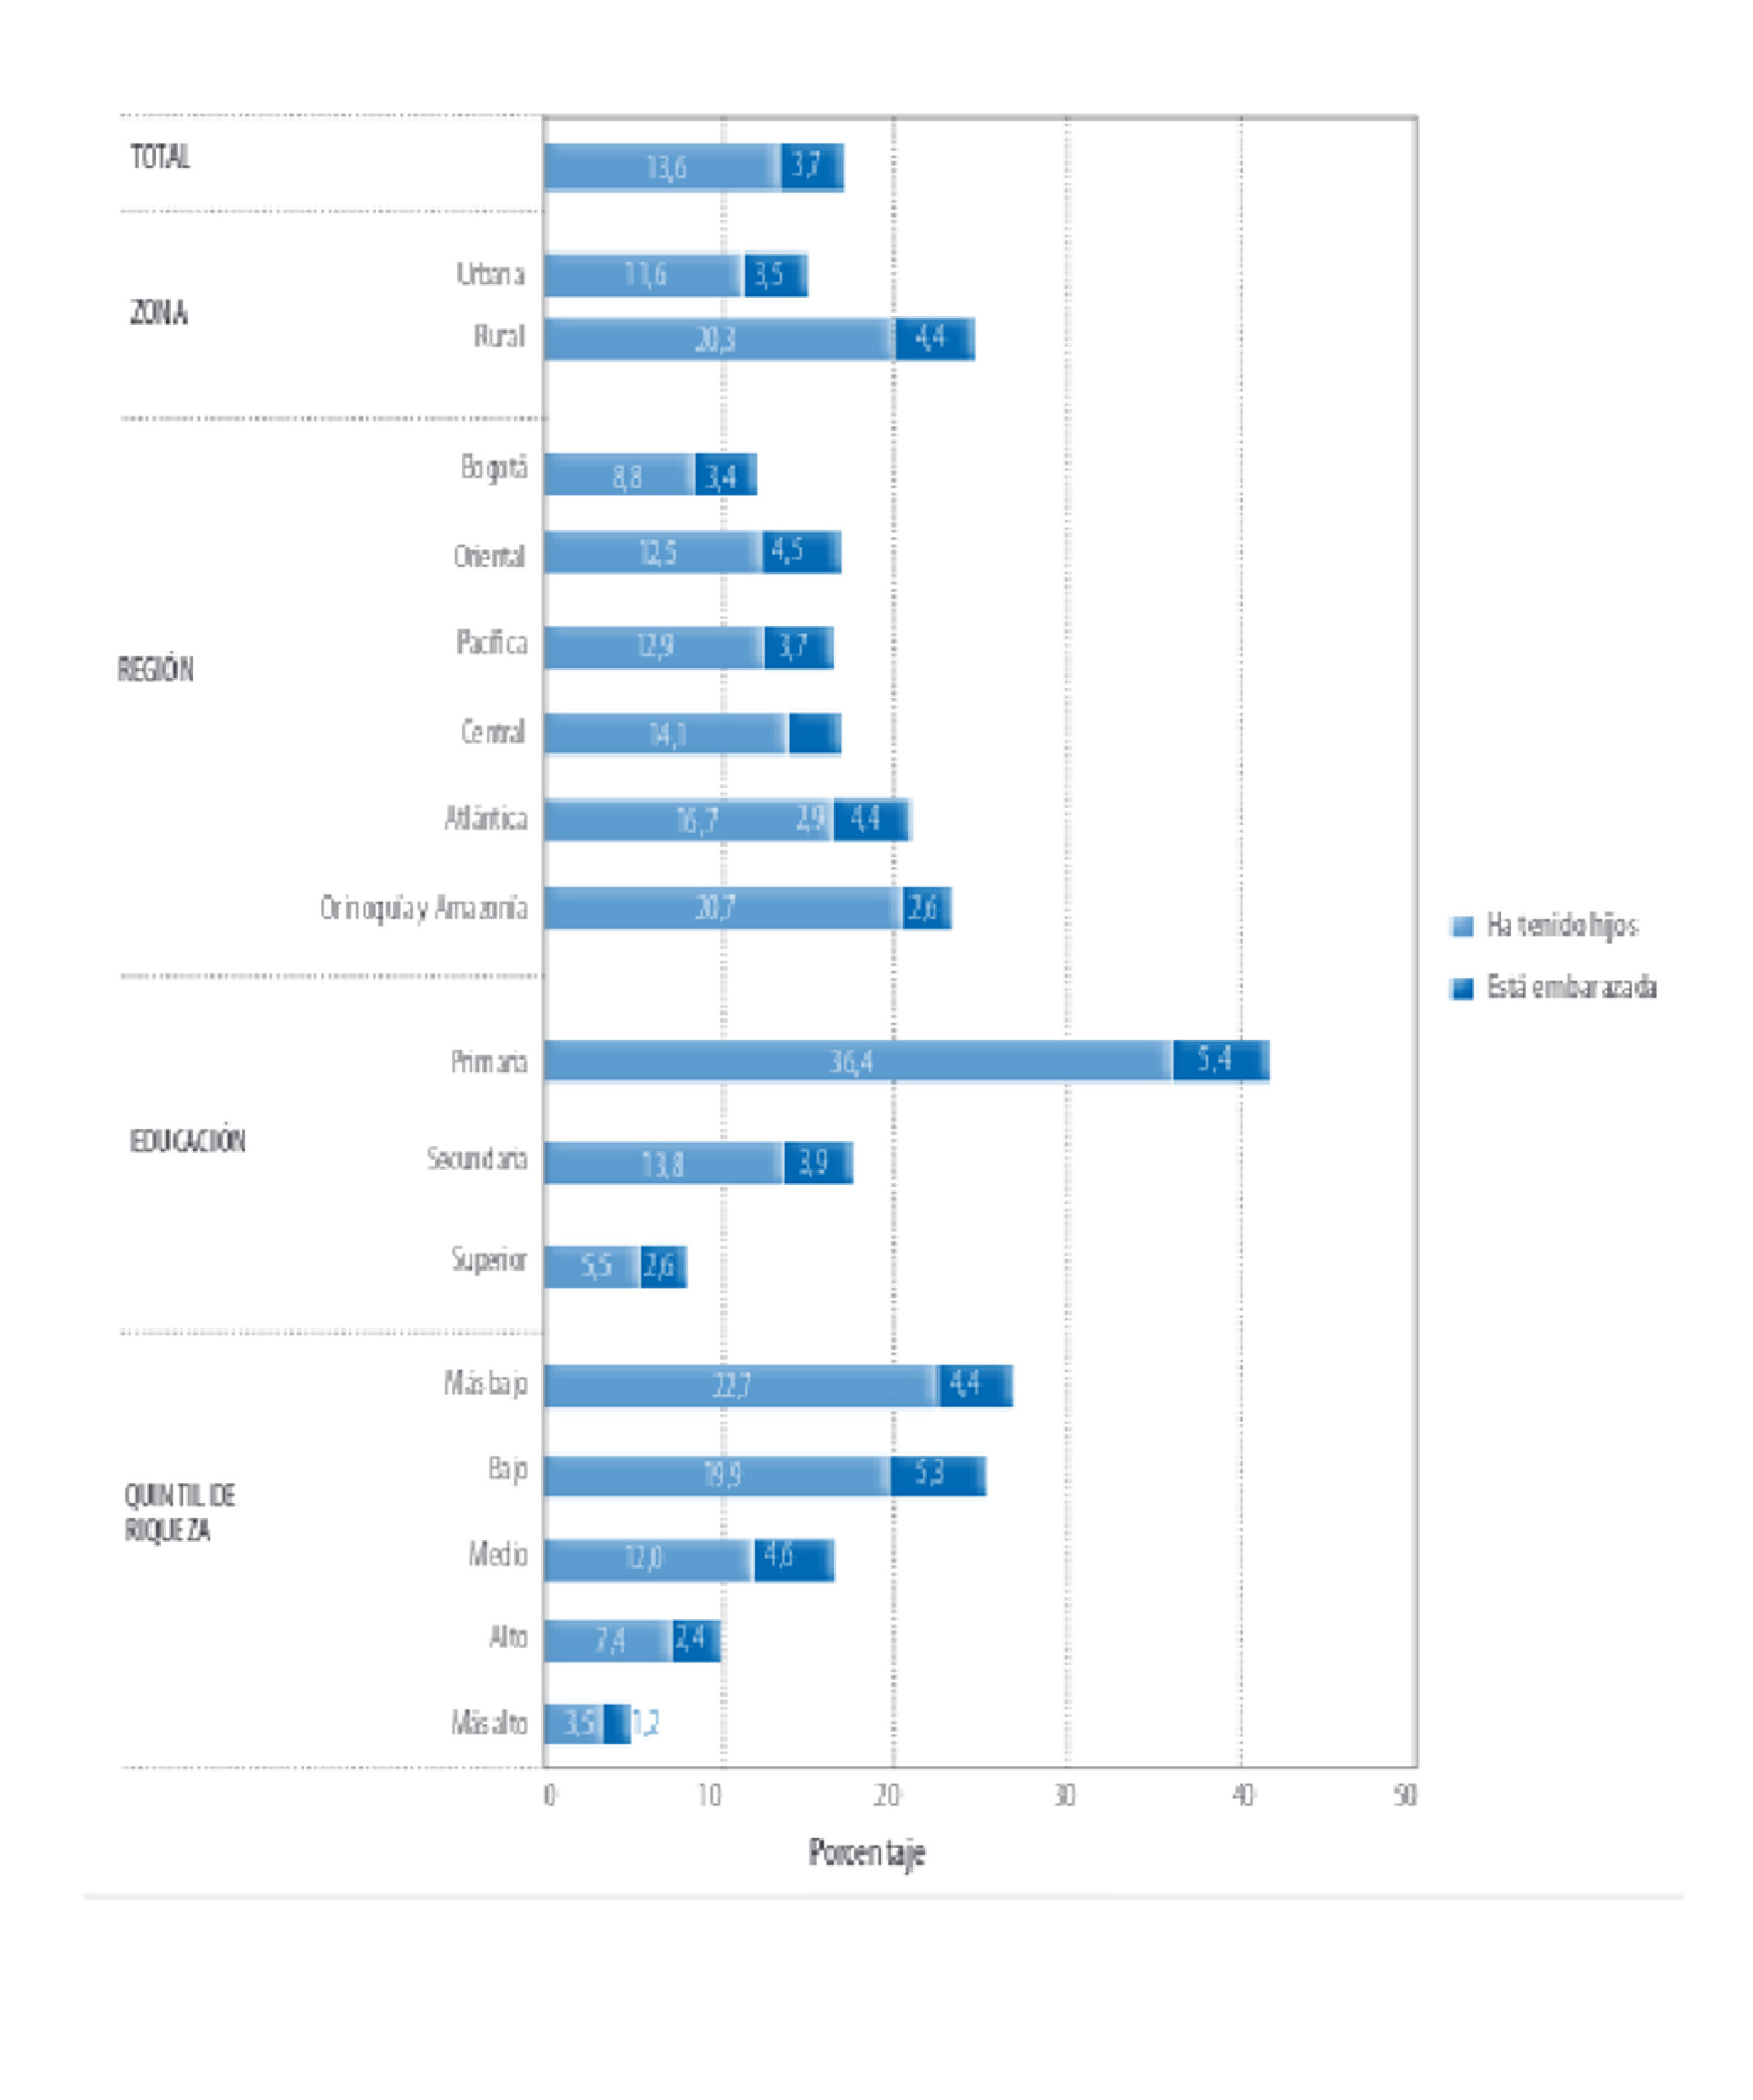
\includegraphics[width=6in,height=3.5in]{datos.eps}
%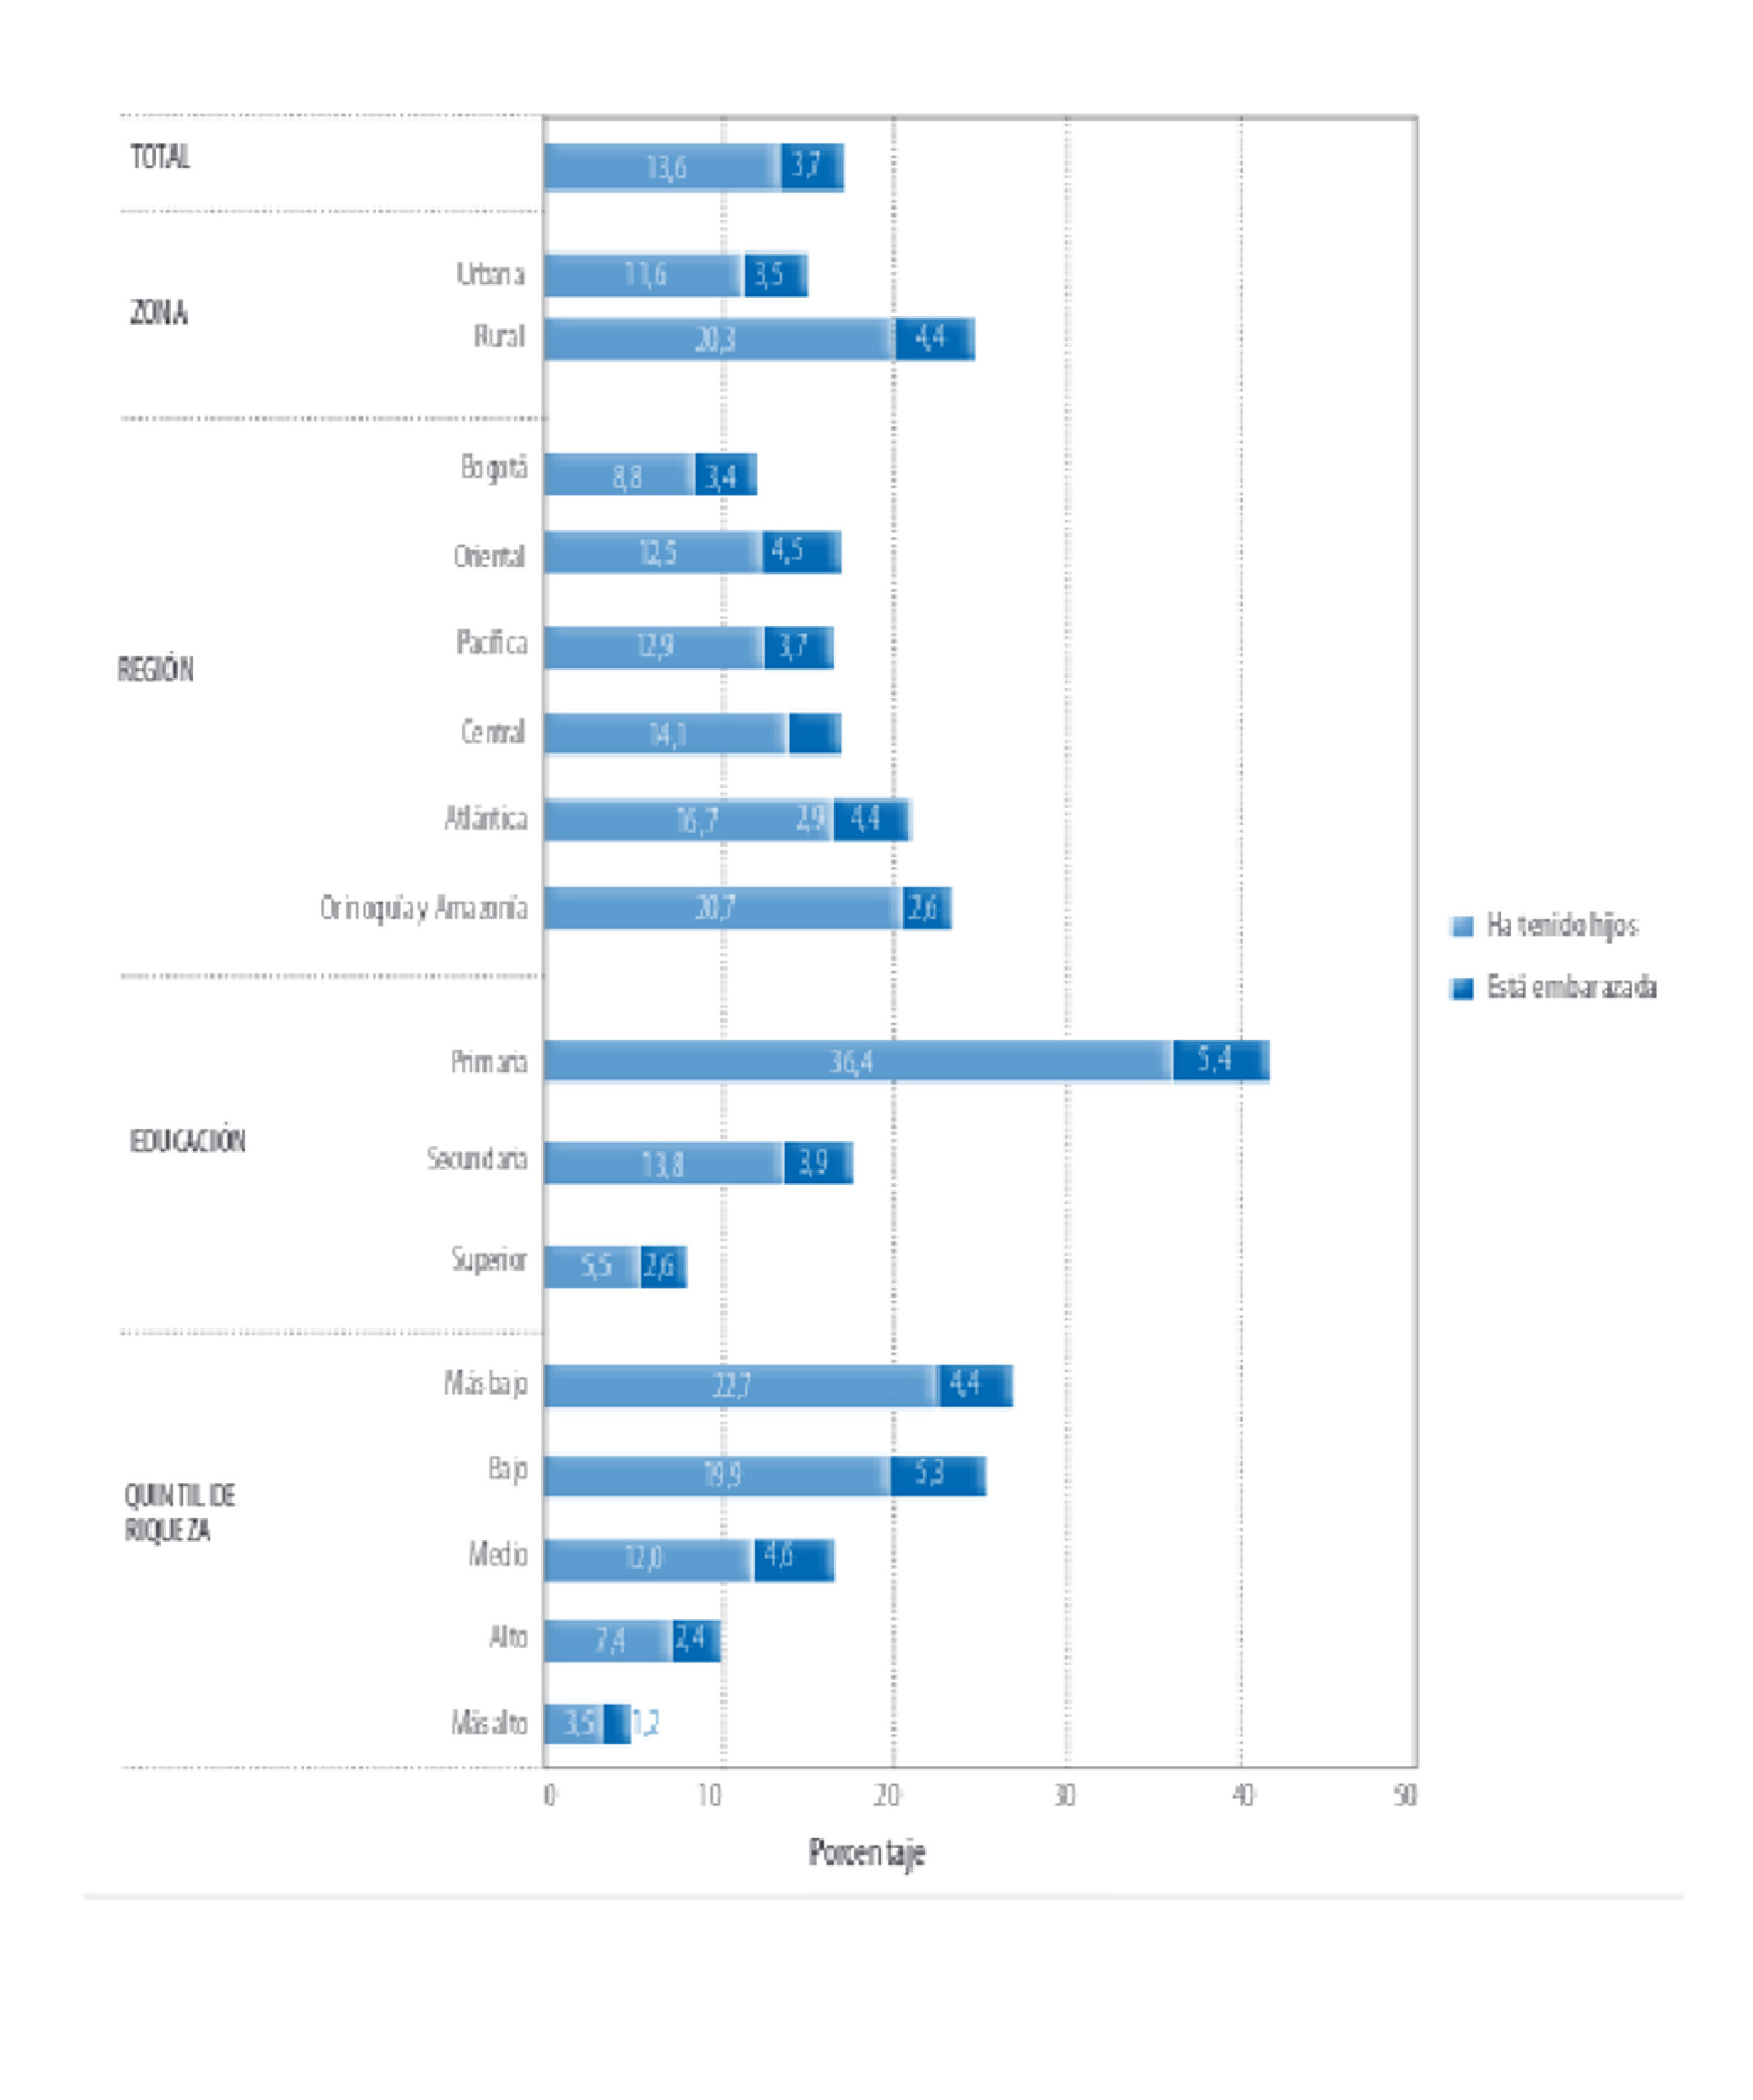
\includegraphics[width=\textwidth]{datos.eps}
\caption{Porcentaje de mujeres de 15-19 años embarazadas~\citep{Pro2015}.}
\label{fig:ends}
\end{figure}

La problemática del embarazo adolescente en Colombia demuestra que solo el $9\%$ de las mujeres y el $5\%$ de los hombres jóvenes consultan los servicios de salud debido a la desconfianza y desconocimiento de este sistema. 

A pesar de que los adolescentes son conscientes de los métodos anticonceptivos, tan sólo una pequeña porción los usan, según cifras de~\citep{Pro2015II} para el rango de edad entre 15-19 años, para las mujeres es alrededor del $30\%$ y en los hombres del $47\%$.

Es importante tener en cuenta que el uso de métodos anticonceptivos no solo es importante para controlar los crecimientos de natalidad del país, sino también el hecho de entender que el uso adecuado de estos puede prevenir infecciones de transmisión sexual. En este sentido, el uso del condón se hace referencia en Colombia como una de las prácticas más seguras para prevenir la transmisión ($85.1\%$ en hombres y $84.4\%$ en mujeres).

Cuando se aborda la problemática desde un enfoque de derechos y para dar respuesta a las necesidades de información sobre la educación en temas de sexualidad y reproducción, es necesario plantear la educación de una manera integral, en el que se potencien y fomenten el empoderamiento y se desarrollen habilidades en los jóvenes desde una perspectiva crítica que les permita tomar decisiones que posibiliten el cumplimiento efectivo de sus derechos sexuales y reproductivos. La sexualidad es un derecho humano, cuya construcción efectiva requiere de procesos o estrategias intencionadas, estructuradas y sistemáticas que faciliten el acceso a información sobre temas referentes a la sexualidad analizada en los diferentes entornos geográficos y socioeconómicos más allá del vivido en la escuela.

En Colombia el derecho a la educación sexual hace parte integral tanto de la Constitución Política de 1991 como de las diversas políticas que desarrollan los acuerdos, pactos, conferencias, convenios y convenciones internacionales ratificados por el Estado. El rol del sector educativo en la promoción y garantía de los Derechos Sexuales y Derechos Reproductivos se destaca a partir de la Resolución 3353 de 1993. Por ende, el carácter obligatorio de la educación sexual en las instituciones educativas se ratifica en el Plan Nacional de Educación Sexual (MEN, 1994) y la Ley General de Educación (Ley  115  de 1994 y Decreto reglamentario 1860). Otros referentes normativos son el documento CONPES Social 147, donde se definen los lineamientos para la prevención del embarazo en la adolescencia, el PDSP 2012-2021 (MSPS, 2014), en el cual  se  establece que la sexualidad es una de las dimensiones priorizadas, es decir, considera este aspecto como fundamental para lograr la salud y el bienestar de todo individuo, sin distinción por sexo, género, etnia, ciclo de vida, nivel socioeconómico o cualquier otro aspecto diferencial~\citep{Pro2015II}, el adolescente tiene derecho a la protección y a la formación integral.

Teniendo todo esto en mente, y con el objetivo de configurar una estrategia que abordara de manera integral, buscando compaginar los factores estructurales y trabajar también en las características individuales de los jóvenes (para permitir fortalecer la construcción del ser y fomentando el empoderamiento de su territorio), que se creo la ``Red Sentir...Con-Ciencia Juvenil''. El proyecto Red Sentir Con-Ciencia Juvenil tiene como objetivo implementar estrategias para prevenir el embarazo adolescente enfocándose en los planes de vida de los jóvenes a través del arte y la tecnología en 6 municipios del oriente antioqueño -Sonsón, Abejorral, San Francisco, Marinilla, San Luis y Argelia-, pretendiendo el desarrollo de una plataforma virtual educativa y recreativa, que incluye componentes para redes sociales, dispositivos móviles y video juegos, donde se enfoca en la educación sexual y en el fortalecimiento de los proyectos que configuran los planes de vida de los jóvenes.

El proyecto trabaja 3 componentes que son: (i) Plataforma Digital, (ii) formación y Socialización y (iii) Mesa Regional. Estos componentes permiten que se accionen estrategias pedagógicas articuladas y basadas en temáticas de sexualidad abordándola desde la tecnología, la memoria y la investigación, con lo cual se logra un direccionamiento pedagógico que produzca procesos educativos integrales, holísticos y significativos. 

Las estrategia de la Red Sentir se basa en trabajar sobre sus determinantes, con los que se puedan lograr cambios en la situación inicial y alcanzar reducciones en las tazas de embarazo adolescente en la región del oriente antioqueño. Esto debido a que se incluye una metodología donde las actividades que se realizan promueven la interacción con los jóvenes y sus entornos, lo cual configura un factor determinante al favorecer una relación de confianza y calidad con el joven por parte de un formador que pueda actuar a nivel motivacional y a su vez sirva de referente y/o modelo. Esto proporciona un ambiente de tranquilidad para los jóvenes, donde ellos se apropien de las temáticas tratadas y les permita interactuar de forma segura para abordar aspectos importantes con el fin de incentivar cambios de comportamiento asertivos.

Para llevar a cabo la estrategia de la Red Sentir y estimando la necesidad de utilizar estrategias digitales se construyó la plataforma digital. Esto al considerar el avance y la evolución constante derivado de las transformaciones causadas por el desarrollo de la civilización electrónica y la revolución científica - tecnológica del sistema educativo se ven necesariamente enmarcados dentro de la llamada ``sociedad del conocimiento'', llamada a producir una revolución que seguramente producirá la implantación generalizada de las nuevas tecnologías de la información y de la comunicación (TIC) que regirán el futuro de los sistemas económicos, la innovación cultural, las interacciones humanas y evidentemente los procesos y circunstancias del aprendizaje y de la educación~\citep{Asin2009}. Por tal motivo se hace imprescindible hablar y pensar TIC's, esto en gran medida en los incrementos cualitativos y cuantitativos de su uso, por tal motivo dentro de los contextos educativos no pueden ser ignoradas, por el contrario se vuelve indispensable buscar e incentivar el acceso y apropiación de las mismas de las generaciones venideras para favorecer y promulgar la participación reflexiva, complementando y generando un pensamiento crítico sobre un adecuado uso de las TIC. 

A pesar del pensamiento que genera las TIC en cuanto a acceso y apropiación, es indiscutible que existen abismales desigualdades en cuanto a la posibilidad de acceso a las tecnologías de la información y la comunicación en America Latina que conforman un punto de partida, esto hace referencia a la brecha digital presentada en dos dimensiones. Por un lado, la brecha internacional existente donde se destaca el rezago latinoamericano respecto al avance de las TIC en los países más desarrollados y por el otro, las desigualdades en los países latinoamericanos relacionados con los ingresos medios, la calidad de vida y los ciclo familiares~\citep{Sunkel2006}. El procedimiento para disminuir la brecha existente en el acceso de la tecnología de la información y la comunicación en la sociedad latinoamericana, es logrando una integración pertinente de la educación con las mismas para lograr usos eficientes. El aprovechamiento, actualización, compenetración y en mayor medida de la apropiación que se de en las TIC dependen del acceso de las mismas y la lecturas que se obtengan del contexto social - cultural presente.

En Colombia, de acuerdo a lo establecido en~\citep{Plan2014}, se busca fomentar el uso, el entendimiento, la apropiación y la interacción de las TIC, con lo que se generaran garantías a la sociedad para acceder a estos servicios, lo que convertirá al país a ser parte activa de la sociedad del conocimiento. Dándole preponderancia al uso de las TIC y vinculando esto con los temas educativos, se logra reducir las brechas socioeconómicas, al brindarle a los jóvenes oportunidades para un desarrollo integral, y que a su vez contribuyen a un mejoramiento de la calidad de vida.

Por tal motivo, al ir relacionado con el plan nacional de desarrollo del país, en el que buscan impulsar el desarrollo de aplicaciones y contenidos digitales con impacto social en el que se fortalezcan las TIC y su rol en la sociedad, que la Red Sentir a través de la plataforma digital pretende llegar a una mayor cantidad de personas, sin importar su ubicación geográfica o su estado socioeconómico por medio de un espacio virtual entretenido y dedicado a la prevención del embarazo a una temprana edad y al fortalecimiento de los planes de vida, en el que puedan aprender, entender y apropiarse de los temas relacionados a la salud sexual, salud reproductiva, derechos sexuales y derechos reproductivos.

Las principales características de la plataforma de la Red Sentir que la hace diferente a otros sitios web o plataformas virtuales identificadas (como las del ministerio de protección y salud del gobierno de Colombia~\citep{PagGob2018} o la de la secretaria de salud de Bogotá en alianza con la Fundación Santa Fe de Bogotá y Profamilia~\citep{Sexperto2018}) son: (i) contenido generado de forma agradable para los adolescentes y jóvenes, (ii) participación activa e interacción entre los jóvenes, (iii) juegos de video para la compresión de la sexualidad, (iv) discreción del entorno virtual para incentivar la participación de los jóvenes al ofrecer la posibilidad de participar de manera anónima y (v) públicos objetivos definidos, esto al desplegar dos interfaces diferentes dependiendo si se es joven o adulto.  

El artículo esta organizado de la siguiente manera: después de la introducción, en la sección~\ref{sec:propositos} se definen los propósitos para los cuales se creó la plataforma digital de la Red Sentir y la descripción de las vinculaciones con las autoridades municipales. En la sección~\ref{sec:herramientas} se especifican las herramientas, tecnologías, arquitecturas y además las configuraciones necesarias para la implementación. La sección~\ref{sec:resultados} se muestran los resultados obtenidos hasta el momento, presentando consigo los diferentes módulos que componen la plataforma y los video juegos elaborados. Finalmente en la última sección~\ref{sec:conclusiones} es dedicada a las conclusiones y las perspectivas de trabajo a futuro.


\section{PROPÓSITO}\label{sec:propositos}
La Plataforma digital de la Red Sentir esta pensada para estar al servicio de las secretarías de salud y educación municipales y departamentales para que se articulen y lo usen como medio de divulgación de sus programas de salud sexual y reproductiva, así mismo con la posibilidad de utilizar las guías didácticas para soportar con ello la formación por parte de padres y maestros. La plataforma también cuenta con animaciones, videos y dos video juegos para el uso de los adolescentes en plataformas web y móviles. Adicionalmente, la plataforma sirve para la publicación de contenido relacionado con el tema y los reportes de seguimiento del proyecto, así como foros virtuales en temas concernientes a la salud sexual y al proyecto de vida, donde es posible que interactúen adolescentes, maestros, padres y expertos. La plataforma se planteó bajo el formato de Creative Commons, lo cual ha permitido la fácil vinculación de desarrolladores a la plataforma.

El proyecto de la Red Sentir, busca a través de la plataforma vincular y relacionar estrategias digitales que permitan a los usuarios de la misma, intercambiar conceptos y experiencias aprendidas dentro de los semilleros y a su vez puedan continuar con el proceso de aprendizaje y empoderamiento de las temáticas de sexualidad, plan de vida, sueños y reconocimiento del cuerpo como primer territorio. Para llevar esto a cabo se han programado diferentes módulos que posibilitan una constante interacción, entre los diferentes módulos se puede encontrar una visualización diferente dependiendo de la edad del usuario registrado. 
En el caso de que el usuario sea un joven, podrá contar con los siguientes módulos: (i) una línea de tiempo, (ii) servicios amigables, (iii) preguntas frecuentes, (iv) foros, y por último (v) dos video juegos, todo esto con el fin de fomentar y facilitar el acceso a la información de una manera dinámica, confiable y confidencial. Si el usuario registrado es mayor, la visualización de la plataforma es diferente, el mismo cuenta con algunos módulos en común y otros exclusivos, entre los módulos en común se encuentran: (i) foros, y (ii) video juegos, y de manera diferenciada los módulos:  (i) formación, (ii) mesa regional, y (iii) lineabase.

Para la evaluación de los módulos que conforman la plataforma digital se tienen en cuenta varios aspectos que determinan la calidad de un software, como lo es la evaluación del proceso de desarrollo mediante el cual se ha elaborado el sistema y por otra parte la evaluación de la calidad del producto en sí, se dice que un software es de calidad cuando ejecuta las funciones para las que fue creado con un desempeño óptimo.

La plataforma digital de la red sentir requiere de un alto nivel de calidad y seguridad ya que en esta se pretende contener información personal de miles de usuarios, para tener acogida y generar confianza en los usuarios respecto de los tiempos de respuesta y confidencialidad de los datos.

\section{HERRAMIENTAS, TECNOLOGÍAS y CONFIGURACIONES}\label{sec:herramientas}
Teniendo en cuenta el formato de Creative Commons para el que fue pensado la plataforma, y tomando como base el concepto de Software Libre, Python fue seleccionado por su característica OpenSource, por ser un lenguaje de programación dinámico y orientado a objetos, a su integración con otros lenguajes y herramientas y además de ser multiparadigma y multiplataforma.

En la actualidad cualquier aplicación web es la suma de diferentes lenguajes de programación y lenguajes de etiquetado. Esto se debe principalmente a que la web ya no es únicamente un conjunto de páginas HTML estáticas. Se han desarrollado distintas tecnologías que han permitido páginas dinámicas y aplicaciones complejas. Esta complejidad hace que sea preciso un diseño cuidadoso y una lógica de aplicación en servidor o cliente que permita al usuario realizar las tareas pertinentes.

\subsection{Servidor web}
El diseño se basa en la ejecución de los programas correspondientes sobre un servidor central HPE Proliant DL120 Gen9~\citep{Manual2018} ubicado en las instalaciones de CORUM, el mismo cuenta con las siguientes características: 
\begin{itemize}
	\item Factor de Forma: Rack (1U)
	\item Procesador: Intel Xeon E5-2603v4 6-Core (1.70GHz 15MB L3 Cache) / Máximo: 1 Procesador
	\item Memoria RAM: 24GB (1 x 16GB + 1 x 8GB) DDR4 2400MHz RDIMM
	\item Ranuras de Memoria: 8 Slots
	\item Gráficos: Integrated Matrox G200eH2
	\item Red: HP Embedded Dual Port 361i Adapter HP Ethernet 331T PCIe 4 Puertos 10/100/1000 Discos Duros: Disco Duro HPE 1TB 6G SATA 7.2k 3.5in SC STND LFF / Máximo: 4 Discos
	\item Controladora de Discos: Dynamic Smart Array B140i controller (No Cache)
	\item Raid: 0/1/1+0/5 Solo SATA (Para SAS agregar controlador adicional)
	\item Placa Conexión De Discos Duros: Hot Plug 3.5in Large Form Factor Smart Carrier Hard Disk
	\item Unidad Óptica: Ninguna / Maximo: 1
	\item Fuente De Alimentación: 1 x Non-Pluggable Non-Redundant 550W FIO Power Supply / Maximo: 2 Fuentes	
\end{itemize}

Para la configuración del servidor se instaló la versión de ubuntu server 16.04.03 LTS Xenial basado en un sistema operativo de linux.

La programación del Servidor se llevó a cabo por medio del framework cherrypy que se explica en la sub-sección~\ref{sub:cherrypy}

Aplicaciones del lado del cliente (client-side): Aquí entra en juego el lenguaje JavaScript y HTML. El servidor proporciona el código y el cliente (mediante el navegador) las ejecuta. 

Aplicaciones en el lado del servidor (server-side):el servidor ejecuta la aplicación; ésta, una vez ejecutada, genera cierto código HTML; el servidor toma este código recién creado y lo enviá al cliente por medio del protocolo HTTP. Para las aplicaciones del lado del servidor, el lenguaje utilizado fue  Python.

Los lenguajes utilizados para cumplir dicha tarea fueron Html, Python (Server-Side), Postgresql y JavaScript (Client-Side). Las librerías utilizadas (todas con licencia GNU)fueron jQuery, Bootstrap, entre otras.

\subsection{Programación}
La Programación de los distintos módulos que conforman la plataforma digital de la Red Sentir utiliza el patrón de arquitectura de software Modelo-Vista-Controlador, empleando para esto el diseño de programación orienta da objetos, con el cual se usa el principio de ``No Te Repitas'' o \textbf{DRY} (por sus siglas en inglés ``Don't Repeat Yourself'') permitiendo con esto un manejo más eficiente de cambios y a su ver proporcionar una mejor sincronización. Aunque con la tecnología usada en este desarrollo lo modifica un poco y lleva a hablar de un patrón Modelo-Vista-Template (MVT) en django. El patrón de programación MVT es análogo, el modelo continua siendo el modelo, en este caso, la vista describe que datos serán presentados, por lo que no configura una vista en si, sino más bien es un controlador que se llama vista, en el caso del template corresponden a las vistas del MVC, es decir, la forma en como son presentados los datos, por lo que los formularios van en template, estos formularios hacen peticiones a las vistas, y a su vez las vistas obtienen datos de los modelos.

\subsubsection{Framework Django}
Django es un framework para desarrollo web de código abierto basado $100\%$ en el lenguaje de programación Python (django esta escrito como una colección de librerías de Python) que utiliza el patrón de programación MVT~\citep{Hol2009, DjangoM}



La meta fundamental de Django es facilitar la creación de sitios web complejos. Django pone énfasis en el re-uso, la conectividad y extensibilidad de componentes, el desarrollo rápido y el principio No te repitas (DRY, del inglés Don't Repeat Yourself). Python es usado en todas las partes del framework, incluso en configuraciones, archivos, y en los modelos de datos. 


\subsubsection{Framework Cherrypy}\label{sub:cherrypy}

\subsection{Base de Datos}
Para trabajar los datos que se manejan en la plataforma se hace por medio de bases de datos relacionales
\subsubsection{Postgres}

\subsection{Video Juego}
Hablar de las diferentes herramientas utilizadas, tales como TexturePacker
\subsubsection{Cocos Creator}

\subsubsection{Ilustraciones}
mirar si se pone esto, pero no sé ni los programas ni la metodología utilizada para la ilustración 

\section{Resultados}\label{sec:resultados}

Resultados: Plataforma digital en funcionamiento, información colgada, juego en funcionamiento, materiales pedagógicos con acceso virtual, enlaces con entidades del sector y aliados.  Sostenibilidad de la plataforma, actualización, noticias, enlaces, participación en foros, respuestas a dudas, motivación a participar.

\section{CONCLUSIONES y PERSPECTIVAS}\label{sec:conclusiones}


\newpage
\bibliographystyle{apa-good}
\bibliography{biblio_digital}
\end{document}